\documentclass{tutkielma}

\title{Tutkielma-tyylin esimerkki}
\author{Asko}{Tapani}{Soukka}
\location{Jyväskylä}
\university{Jyväskylän yliopisto}
\department{Tietojenkäsittelytieteiden laitos}
\subject{Tietojärjestelmätieteen}
\type{Esimerkki}
\keywords{\LaTeX, taitto}

%\fixdate{13}{7}{2007}

\usepackage{texnames}
\usepackage[pdftex]{graphicx}

\begin{document}

\maketitle

\begin{abstract}

Tämä on esimerkki tutkielma"-tyylin käytöstä.

\end{abstract}

\tableofcontents

\chapter{Esimerkkiluku}

\section{Esimerkkiluvun alaluku}

\subsection{Esimerkkiluvun alaluvun alaluku}

Tutkielma"-tyyli on laadittu noudattaen Puurosen ohjeita \citep{Puuronen2002Ohjeita-tutkimusraportin-kirjoittajalle}. Kun vuodenvaihteessa 2006--2007 kysyin itse Puuroselta kommentteja silloin nopeimmassa kehitysvaiheessa olleeseen tyyliini, hän suositteli aloittamaan kappaleet kuvioiden \figref[esim.][]{fig:Kuvioita} ja taulukoiden \tabref[esim.][]{tbl:Hypertekstin-historiaa} jälkeen aivan vasemmasta marginaalista.

\begin{table}[h!]
\caption[Hypertekstin historiaa]{Hypertekstin historiaa \citep[6--9]{Heimburg1989Hyperjarjestelmat}.}
\centering
\begin{tabular}{lll}
    1945        & Bush V.                   & Memex                     \\
    1960        & Engelbart D.              & NLS/Augment               \\
    1960        & Nelson, T.H.              & Xanadu                    \\
    1967--1968  & Nelson ja van Dam, A.       & Hypertext Editing System  \\
    1975        & van Dam                   & FRESS                     \\
    1982        & Brown University / IRIS   & Electronic Document System\\
    1985        & Meyrowitz, N. ja Yankelovich, N. & Intermedia          \\
    1987        & Strassman, P.             & NoteCards                 \\
    1987        & Brown, P.                 & Guide                     \\
    1987        & Atkinson, B.              & HyperCard                 \\
\end{tabular}
\label{tbl:Hypertekstin-historiaa}
\end{table}

\noindent Tyyli sisältää tuen \emph{subfigure}"-paketille, jonka avulla yhden viitattavan kuvion \figref[esim.][]{fig:Kuvioita} voi koostaa useasta osakuviosta \figref[esim.][a--b]{fig:Kuvioita}.

\begin{figure}[h]
\subfigure[Ekakuva]{
  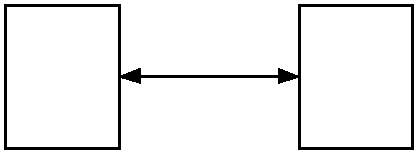
\includegraphics[width=6.75cm]{kuviot/ekakuvio.pdf}
}
\hspace{0.75cm}
\subfigure[Tokakuva]{
  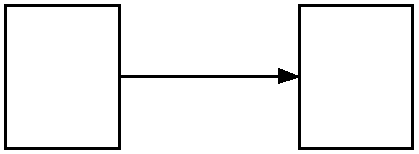
\includegraphics[width=6.75cm]{kuviot/tokakuvio.pdf}
}
\caption[Kuvioita]{Kuvioita.}
\label{fig:Kuvioita}
\end{figure}


\bibliography{esimerkki.bib}

\appendix

\chapter{Ensimmäinen liite}

Lopuksi haluan kiittää Antti"-Jukka Kaijanahoa mainiosta \LaTeX"-oppaastaan \citep{Kaijanaho1998Opus-asiatekstin-ladonnasta}.

\end{document}